
%% bare_jrnl_compsoc.tex
%% V1.3
%% 2007/01/11
%% by Michael Shell
%% See:
%% http://www.michaelshell.org/
%% for current contact information.
%%
%% This is a skeleton file demonstrating the use of IEEEtran.cls
%% (requires IEEEtran.cls version 1.7 or later) with an IEEE Computer
%% Society journal paper.
%%
%% Support sites:
%% http://www.michaelshell.org/tex/ieeetran/
%% http://www.ctan.org/tex-archive/macros/latex/contrib/IEEEtran/
%% and
%% http://www.ieee.org/

%%*************************************************************************
%% Legal Notice:
%% This code is offered as-is without any warranty either expressed or
%% implied; without even the implied warranty of MERCHANTABILITY or
%% FITNESS FOR A PARTICULAR PURPOSE!
%% User assumes all risk.
%% In no event shall IEEE or any contributor to this code be liable for
%% any damages or losses, including, but not limited to, incidental,
%% consequential, or any other damages, resulting from the use or misuse
%% of any information contained here.
%%
%% All comments are the opinions of their respective authors and are not
%% necessarily endorsed by the IEEE.
%%
%% This work is distributed under the LaTeX Project Public License (LPPL)
%% ( http://www.latex-project.org/ ) version 1.3, and may be freely used,
%% distributed and modified. A copy of the LPPL, version 1.3, is included
%% in the base LaTeX documentation of all distributions of LaTeX released
%% 2003/12/01 or later.
%% Retain all contribution notices and credits.
%% ** Modified files should be clearly indicated as such, including  **
%% ** renaming them and changing author support contact information. **
%%
%% File list of work: IEEEtran.cls, IEEEtran_HOWTO.pdf, bare_adv.tex,
%%                    bare_conf.tex, bare_jrnl.tex, bare_jrnl_compsoc.tex
%%*************************************************************************

% *** Authors should verify (and, if needed, correct) their LaTeX system  ***
% *** with the testflow diagnostic prior to trusting their LaTeX platform ***
% *** with production work. IEEE's font choices can trigger bugs that do  ***
% *** not appear when using other class files.                            ***
% The testflow support page is at:
% http://www.michaelshell.org/tex/testflow/




% Note that the a4paper option is mainly intended so that authors in
% countries using A4 can easily print to A4 and see how their papers will
% look in print - the typesetting of the document will not typically be
% affected with changes in paper size (but the bottom and side margins will).
% Use the testflow package mentioned above to verify correct handling of
% both paper sizes by the user's LaTeX system.
%
% Also note that the "draftcls" or "draftclsnofoot", not "draft", option
% should be used if it is desired that the figures are to be displayed in
% draft mode.
%
% The Computer Society usually requires 10pt for submissions.
%
\documentclass[10pt,journal,cspaper,compsoc]{IEEEtran}
%
% If IEEEtran.cls has not been installed into the LaTeX system files,
% manually specify the path to it like:
% \documentclass[12pt,journal,compsoc]{../sty/IEEEtran}





% Some very useful LaTeX packages include:
% (uncomment the ones you want to load)


% *** MISC UTILITY PACKAGES ***
%
%\usepackage{ifpdf}
% Heiko Oberdiek's ifpdf.sty is very useful if you need conditional
% compilation based on whether the output is pdf or dvi.
% usage:
% \ifpdf
%   % pdf code
% \else
%   % dvi code
% \fi
% The latest version of ifpdf.sty can be obtained from:
% http://www.ctan.org/tex-archive/macros/latex/contrib/oberdiek/
% Also, note that IEEEtran.cls V1.7 and later provides a builtin
% \ifCLASSINFOpdf conditional that works the same way.
% When switching from latex to pdflatex and vice-versa, the compiler may
% have to be run twice to clear warning/error messages.






% *** CITATION PACKAGES ***
%
\ifCLASSOPTIONcompsoc
  % IEEE Computer Society needs nocompress option
  % requires cite.sty v4.0 or later (November 2003)
  \usepackage[nocompress]{cite}
\else
  % normal IEEE
  % \usepackage{cite}
\fi
% cite.sty was written by Donald Arseneau
% V1.6 and later of IEEEtran pre-defines the format of the cite.sty package
% \cite{} output to follow that of IEEE. Loading the cite package will
% result in citation numbers being automatically sorted and properly
% "compressed/ranged". e.g., [1], [9], [2], [7], [5], [6] without using
% cite.sty will become [1], [2], [5]--[7], [9] using cite.sty. cite.sty's
% \cite will automatically add leading space, if needed. Use cite.sty's
% noadjust option (cite.sty V3.8 and later) if you want to turn this off.
% cite.sty is already installed on most LaTeX systems. Be sure and use
% version 4.0 (2003-05-27) and later if using hyperref.sty. cite.sty does
% not currently provide for hyperlinked citations.
% The latest version can be obtained at:
% http://www.ctan.org/tex-archive/macros/latex/contrib/cite/
% The documentation is contained in the cite.sty file itself.
%
% Note that some packages require special options to format as the Computer
% Society requires. In particular, Computer Society  papers do not use
% compressed citation ranges as is done in typical IEEE papers
% (e.g., [1]-[4]). Instead, they list every citation separately in order
% (e.g., [1], [2], [3], [4]). To get the latter we need to load the cite
% package with the nocompress option which is supported by cite.sty v4.0
% and later. Note also the use of a CLASSOPTION conditional provided by
% IEEEtran.cls V1.7 and later.





% *** GRAPHICS RELATED PACKAGES ***
%
\ifCLASSINFOpdf
   \usepackage[pdftex]{graphicx}
   \usepackage{epstopdf}
  % declare the path(s) where your graphic files are
  % \graphicspath{{../pdf/}{../jpeg/}}
  \graphicspath{{./fig/}}
  % and their extensions so you won't have to specify these with
  % every instance of \includegraphics
  % \DeclareGraphicsExtensions{.pdf,.jpeg,.png,.eps}
\else
  % or other class option (dvipsone, dvipdf, if not using dvips). graphicx
  % will default to the driver specified in the system graphics.cfg if no
  % driver is specified.
   \usepackage[dvips]{graphicx}
  % declare the path(s) where your graphic files are
  % \graphicspath{{../eps/}}
  \graphicspath{{./fig/}}
  % and their extensions so you won't have to specify these with
  % every instance of \includegraphics
   \DeclareGraphicsExtensions{.eps}
\fi
% graphicx was written by David Carlisle and Sebastian Rahtz. It is
% required if you want graphics, photos, etc. graphicx.sty is already
% installed on most LaTeX systems. The latest version and documentation can
% be obtained at:
% http://www.ctan.org/tex-archive/macros/latex/required/graphics/
% Another good source of documentation is "Using Imported Graphics in
% LaTeX2e" by Keith Reckdahl which can be found as epslatex.ps or
% epslatex.pdf at: http://www.ctan.org/tex-archive/info/
%
% latex, and pdflatex in dvi mode, support graphics in encapsulated
% postscript (.eps) format. pdflatex in pdf mode supports graphics
% in .pdf, .jpeg, .png and .mps (metapost) formats. Users should ensure
% that all non-photo figures use a vector format (.eps, .pdf, .mps) and
% not a bitmapped formats (.jpeg, .png). IEEE frowns on bitmapped formats
% which can result in "jaggedy"/blurry rendering of lines and letters as
% well as large increases in file sizes.
%
% You can find documentation about the pdfTeX application at:
% http://www.tug.org/applications/pdftex





% *** MATH PACKAGES ***
%
\usepackage[cmex10]{amsmath}
% A popular package from the American Mathematical Society that provides
% many useful and powerful commands for dealing with mathematics. If using
% it, be sure to load this package with the cmex10 option to ensure that
% only type 1 fonts will utilized at all point sizes. Without this option,
% it is possible that some math symbols, particularly those within
% footnotes, will be rendered in bitmap form which will result in a
% document that can not be IEEE Xplore compliant!
%
% Also, note that the amsmath package sets \interdisplaylinepenalty to 10000
% thus preventing page breaks from occurring within multiline equations. Use:
%\interdisplaylinepenalty=2500
% after loading amsmath to restore such page breaks as IEEEtran.cls normally
% does. amsmath.sty is already installed on most LaTeX systems. The latest
% version and documentation can be obtained at:
% http://www.ctan.org/tex-archive/macros/latex/required/amslatex/math/





% *** SPECIALIZED LIST PACKAGES ***
%
%\usepackage{algorithmic}
% algorithmic.sty was written by Peter Williams and Rogerio Brito.
% This package provides an algorithmic environment fo describing algorithms.
% You can use the algorithmic environment in-text or within a figure
% environment to provide for a floating algorithm. Do NOT use the algorithm
% floating environment provided by algorithm.sty (by the same authors) or
% algorithm2e.sty (by Christophe Fiorio) as IEEE does not use dedicated
% algorithm float types and packages that provide these will not provide
% correct IEEE style captions. The latest version and documentation of
% algorithmic.sty can be obtained at:
% http://www.ctan.org/tex-archive/macros/latex/contrib/algorithms/
% There is also a support site at:
% http://algorithms.berlios.de/index.html
% Also of interest may be the (relatively newer and more customizable)
% algorithmicx.sty package by Szasz Janos:
% http://www.ctan.org/tex-archive/macros/latex/contrib/algorithmicx/

\usepackage[normalem]{ulem}
\usepackage[linesnumbered,boxed,commentsnumbered,ruled]{algorithm2e}






% *** ALIGNMENT PACKAGES ***
%
%\usepackage{array}
% Frank Mittelbach's and David Carlisle's array.sty patches and improves
% the standard LaTeX2e array and tabular environments to provide better
% appearance and additional user controls. As the default LaTeX2e table
% generation code is lacking to the point of almost being broken with
% respect to the quality of the end results, all users are strongly
% advised to use an enhanced (at the very least that provided by array.sty)
% set of table tools. array.sty is already installed on most systems. The
% latest version and documentation can be obtained at:
% http://www.ctan.org/tex-archive/macros/latex/required/tools/


%\usepackage{mdwmath}
%\usepackage{mdwtab}
% Also highly recommended is Mark Wooding's extremely powerful MDW tools,
% especially mdwmath.sty and mdwtab.sty which are used to format equations
% and tables, respectively. The MDWtools set is already installed on most
% LaTeX systems. The lastest version and documentation is available at:
% http://www.ctan.org/tex-archive/macros/latex/contrib/mdwtools/


% IEEEtran contains the IEEEeqnarray family of commands that can be used to
% generate multiline equations as well as matrices, tables, etc., of high
% quality.


%\usepackage{eqparbox}
% Also of notable interest is Scott Pakin's eqparbox package for creating
% (automatically sized) equal width boxes - aka "natural width parboxes".
% Available at:
% http://www.ctan.org/tex-archive/macros/latex/contrib/eqparbox/





% *** SUBFIGURE PACKAGES ***
%\ifCLASSOPTIONcompsoc
%\usepackage[tight,normalsize,sf,SF]{subfigure}
%\else
%\usepackage[tight,footnotesize]{subfigure}
%\fi
% subfigure.sty was written by Steven Douglas Cochran. This package makes it
% easy to put subfigures in your figures. e.g., "Figure 1a and 1b". For IEEE
% work, it is a good idea to load it with the tight package option to reduce
% the amount of white space around the subfigures. Computer Society papers
% use a larger font and \sffamily font for their captions, hence the
% additional options needed under compsoc mode. subfigure.sty is already
% installed on most LaTeX systems. The latest version and documentation can
% be obtained at:
% http://www.ctan.org/tex-archive/obsolete/macros/latex/contrib/subfigure/
% subfigure.sty has been superceeded by subfig.sty.


%\ifCLASSOPTIONcompsoc
%  \usepackage[caption=false]{caption}
%  \usepackage[font=normalsize,labelfont=sf,textfont=sf]{subfig}
%\else
%  \usepackage[caption=false]{caption}
%  \usepackage[font=footnotesize]{subfig}
%\fi
% subfig.sty, also written by Steven Douglas Cochran, is the modern
% replacement for subfigure.sty. However, subfig.sty requires and
% automatically loads Axel Sommerfeldt's caption.sty which will override
% IEEEtran.cls handling of captions and this will result in nonIEEE style
% figure/table captions. To prevent this problem, be sure and preload
% caption.sty with its "caption=false" package option. This is will preserve
% IEEEtran.cls handing of captions. Version 1.3 (2005/06/28) and later
% (recommended due to many improvements over 1.2) of subfig.sty supports
% the caption=false option directly:
%\ifCLASSOPTIONcompsoc
%  \usepackage[caption=false,font=normalsize,labelfont=sf,textfont=sf]{subfig}
%\else
%  \usepackage[caption=false,font=footnotesize]{subfig}
%\fi
%
% The latest version and documentation can be obtained at:
% http://www.ctan.org/tex-archive/macros/latex/contrib/subfig/
% The latest version and documentation of caption.sty can be obtained at:
% http://www.ctan.org/tex-archive/macros/latex/contrib/caption/




% *** FLOAT PACKAGES ***
%
\usepackage{fixltx2e}
% fixltx2e, the successor to the earlier fix2col.sty, was written by
% Frank Mittelbach and David Carlisle. This package corrects a few problems
% in the LaTeX2e kernel, the most notable of which is that in current
% LaTeX2e releases, the ordering of single and double column floats is not
% guaranteed to be preserved. Thus, an unpatched LaTeX2e can allow a
% single column figure to be placed prior to an earlier double column
% figure. The latest version and documentation can be found at:
% http://www.ctan.org/tex-archive/macros/latex/base/



%\usepackage{stfloats}
% stfloats.sty was written by Sigitas Tolusis. This package gives LaTeX2e
% the ability to do double column floats at the bottom of the page as well
% as the top. (e.g., "\begin{figure*}[!b]" is not normally possible in
% LaTeX2e). It also provides a command:
%\fnbelowfloat
% to enable the placement of footnotes below bottom floats (the standard
% LaTeX2e kernel puts them above bottom floats). This is an invasive package
% which rewrites many portions of the LaTeX2e float routines. It may not work
% with other packages that modify the LaTeX2e float routines. The latest
% version and documentation can be obtained at:
% http://www.ctan.org/tex-archive/macros/latex/contrib/sttools/
% Documentation is contained in the stfloats.sty comments as well as in the
% presfull.pdf file. Do not use the stfloats baselinefloat ability as IEEE
% does not allow \baselineskip to stretch. Authors submitting work to the
% IEEE should note that IEEE rarely uses double column equations and
% that authors should try to avoid such use. Do not be tempted to use the
% cuted.sty or midfloat.sty packages (also by Sigitas Tolusis) as IEEE does
% not format its papers in such ways.




%\ifCLASSOPTIONcaptionsoff
%  \usepackage[nomarkers]{endfloat}
% \let\MYoriglatexcaption\caption
% \renewcommand{\caption}[2][\relax]{\MYoriglatexcaption[#2]{#2}}
%\fi
% endfloat.sty was written by James Darrell McCauley and Jeff Goldberg.
% This package may be useful when used in conjunction with IEEEtran.cls'
% captionsoff option. Some IEEE journals/societies require that submissions
% have lists of figures/tables at the end of the paper and that
% figures/tables without any captions are placed on a page by themselves at
% the end of the document. If needed, the draftcls IEEEtran class option or
% \CLASSINPUTbaselinestretch interface can be used to increase the line
% spacing as well. Be sure and use the nomarkers option of endfloat to
% prevent endfloat from "marking" where the figures would have been placed
% in the text. The two hack lines of code above are a slight modification of
% that suggested by in the endfloat docs (section 8.3.1) to ensure that
% the full captions always appear in the list of figures/tables - even if
% the user used the short optional argument of \caption[]{}.
% IEEE papers do not typically make use of \caption[]'s optional argument,
% so this should not be an issue. A similar trick can be used to disable
% captions of packages such as subfig.sty that lack options to turn off
% the subcaptions:
% For subfig.sty:
% \let\MYorigsubfloat\subfloat
% \renewcommand{\subfloat}[2][\relax]{\MYorigsubfloat[]{#2}}
% For subfigure.sty:
% \let\MYorigsubfigure\subfigure
% \renewcommand{\subfigure}[2][\relax]{\MYorigsubfigure[]{#2}}
% However, the above trick will not work if both optional arguments of
% the \subfloat/subfig command are used. Furthermore, there needs to be a
% description of each subfigure *somewhere* and endfloat does not add
% subfigure captions to its list of figures. Thus, the best approach is to
% avoid the use of subfigure captions (many IEEE journals avoid them anyway)
% and instead reference/explain all the subfigures within the main caption.
% The latest version of endfloat.sty and its documentation can obtained at:
% http://www.ctan.org/tex-archive/macros/latex/contrib/endfloat/
%
% The IEEEtran \ifCLASSOPTIONcaptionsoff conditional can also be used
% later in the document, say, to conditionally put the References on a
% page by themselves.




% *** PDF, URL AND HYPERLINK PACKAGES ***
%
\usepackage{url}
% url.sty was written by Donald Arseneau. It provides better support for
% handling and breaking URLs. url.sty is already installed on most LaTeX
% systems. The latest version can be obtained at:
% http://www.ctan.org/tex-archive/macros/latex/contrib/misc/
% Read the url.sty source comments for usage information. Basically,
% \url{my_url_here}.





% *** Do not adjust lengths that control margins, column widths, etc. ***
% *** Do not use packages that alter fonts (such as pslatex).         ***
% There should be no need to do such things with IEEEtran.cls V1.6 and later.
% (Unless specifically asked to do so by the journal or conference you plan
% to submit to, of course. )


% correct bad hyphenation here
\hyphenation{op-tical net-works semi-conduc-tor}


\begin{document}
%
% paper title
% can use linebreaks \\ within to get better formatting as desired
\title{Measuring the Differences of Large Program Traces Based-on
Levenshtein Distance}
%
%
% author names and IEEE memberships
% note positions of commas and nonbreaking spaces ( ~ ) LaTeX will not break
% a structure at a ~ so this keeps an author's name from being broken across
% two lines.
% use \thanks{} to gain access to the first footnote area
% a separate \thanks must be used for each paragraph as LaTeX2e's \thanks
% was not built to handle multiple paragraphs
%
%
%\IEEEcompsocitemizethanks is a special \thanks that produces the bulleted
% lists the Computer Society journals use for "first footnote" author
% affiliations. Use \IEEEcompsocthanksitem which works much like \item
% for each affiliation group. When not in compsoc mode,
% \IEEEcompsocitemizethanks becomes like \thanks and
% \IEEEcompsocthanksitem becomes a line break with idention. This
% facilitates dual compilation, although admittedly the differences in the
% desired content of \author between the different types of papers makes a
% one-size-fits-all approach a daunting prospect. For instance, compsoc
% journal papers have the author affiliations above the "Manuscript
% received ..."  text while in non-compsoc journals this is reversed. Sigh.

%\author{Michael~Shell,~\IEEEmembership{Member,~IEEE,}
%        John~Doe,~\IEEEmembership{Fellow,~OSA,}
%        and~Jane~Doe,~\IEEEmembership{Life~Fellow,~IEEE}% <-this % stops a space
%\IEEEcompsocitemizethanks{\IEEEcompsocthanksitem M. Shell is with the Department
%of Electrical and Computer Engineering, Georgia Institute of Technology, Atlanta,
%GA, 30332.\protect\\
% note need leading \protect in front of \\ to get a newline within \thanks as
% \\ is fragile and will error, could use \hfil\break instead.
%E-mail: see http://www.michaelshell.org/contact.html
%\IEEEcompsocthanksitem J. Doe and J. Doe are with Anonymous University.}% <-this % stops a space
%\thanks{}}

% note the % following the last \IEEEmembership and also \thanks -
% these prevent an unwanted space from occurring between the last author name
% and the end of the author line. i.e., if you had this:
%
% \author{....lastname \thanks{...} \thanks{...} }
%                     ^------------^------------^----Do not want these spaces!
%
% a space would be appended to the last name and could cause every name on that
% line to be shifted left slightly. This is one of those "LaTeX things". For
% instance, "\textbf{A} \textbf{B}" will typeset as "A B" not "AB". To get
% "AB" then you have to do: "\textbf{A}\textbf{B}"
% \thanks is no different in this regard, so shield the last } of each \thanks
% that ends a line with a % and do not let a space in before the next \thanks.
% Spaces after \IEEEmembership other than the last one are OK (and needed) as
% you are supposed to have spaces between the names. For what it is worth,
% this is a minor point as most people would not even notice if the said evil
% space somehow managed to creep in.



% The paper headers
\markboth{Journal of \LaTeX\ Class Files,~Vol.~6, No.~1, January~2007}%
{Shell \MakeLowercase{\textit{et al.}}: Bare Demo of IEEEtran.cls for Computer Society Journals}
% The only time the second header will appear is for the odd numbered pages
% after the title page when using the twoside option.
%
% *** Note that you probably will NOT want to include the author's ***
% *** name in the headers of peer review papers.                   ***
% You can use \ifCLASSOPTIONpeerreview for conditional compilation here if
% you desire.



% The publisher's ID mark at the bottom of the page is less important with
% Computer Society journal papers as those publications place the marks
% outside of the main text columns and, therefore, unlike regular IEEE
% journals, the available text space is not reduced by their presence.
% If you want to put a publisher's ID mark on the page you can do it like
% this:
%\IEEEpubid{0000--0000/00\$00.00~\copyright~2007 IEEE}
% or like this to get the Computer Society new two part style.
%\IEEEpubid{\makebox[\columnwidth]{\hfill 0000--0000/00/\$00.00~\copyright~2007 IEEE}%
%\hspace{\columnsep}\makebox[\columnwidth]{Published by the IEEE Computer Society\hfill}}
% Remember, if you use this you must call \IEEEpubidadjcol in the second
% column for its text to clear the IEEEpubid mark (Computer Society jorunal
% papers don't need this extra clearance.)




% for Computer Society papers, we must declare the abstract and index terms
% PRIOR to the title within the \IEEEcompsoctitleabstractindextext IEEEtran
% command as these need to go into the title area created by \maketitle.
\IEEEcompsoctitleabstractindextext{%
\begin{abstract}
%\boldmath
Program traces play an important role in analyzing and understanding
program behavior. However, large instruction traces are composed of
millions of instructions, which in turn hinders their effective
analysis. In this paper, we present an efficient algorithm based-on
Levenshtein distance to measure the differences of large traces.
This algorithm calculates the similarity of two traces and
reconstructs the edit sequences, so that users know how similar the
two traces are and where the difference is. We apply our algorithm
to real program traces collected by a pin-tool and a full system
simulator GEM5. Experimental results show that our traces comparison
algorithm is efficient and scalable.
\end{abstract}

% IEEEtran.cls defaults to using nonbold math in the Abstract.
% This preserves the distinction between vectors and scalars. However,
% if the journal you are submitting to favors bold math in the abstract,
% then you can use LaTeX's standard command \boldmath at the very start
% of the abstract to achieve this. Many IEEE journals frown on math
% in the abstract anyway. In particular, the Computer Society does
% not want either math or citations to appear in the abstract.

% Note that keywords are not normally used for peer review papers.
\begin{keywords}
Edit distance, program trace, pin-tool.
\end{keywords}}


% make the title area
\maketitle


% To allow for easy dual compilation without having to reenter the
% abstract/keywords data, the \IEEEcompsoctitleabstractindextext text will
% not be used in maketitle, but will appear (i.e., to be "transported")
% here as \IEEEdisplaynotcompsoctitleabstractindextext when compsoc mode
% is not selected <OR> if conference mode is selected - because compsoc
% conference papers position the abstract like regular (non-compsoc)
% papers do!
\IEEEdisplaynotcompsoctitleabstractindextext
% \IEEEdisplaynotcompsoctitleabstractindextext has no effect when using
% compsoc under a non-conference mode.


% For peer review papers, you can put extra information on the cover
% page as needed:
% \ifCLASSOPTIONpeerreview
% \begin{center} \bfseries EDICS Category: 3-BBND \end{center}
% \fi
%
% For peerreview papers, this IEEEtran command inserts a page break and
% creates the second title. It will be ignored for other modes.
\IEEEpeerreviewmaketitle



\section{Introduction}
Instruction trace characterizes a program's dynamic behavior and is
widely used for program optimization, debugging and new architecture
evaluation. The comparison of program traces reveals important
information about the behavior of two executions. However, low level
program traces, such as instruction sequences, tend to be
considerably large and usually contain millions of instructions,
which in turn hinders their effective analysis. Some existing trace
analysis tools work on high level program traces, such as control
flow graph, call graph and internal event sequences, and rely on
visualization techniques to help software engineers make sense of
trace
content~\cite{trace11}~\cite{trace05}~\cite{trace99}~\cite{trace06}~\cite{trace052}.
Intel Trace Analyzer and Collector is a powerful tool for
understanding MPI application behavior~\cite{traceintel}. It
includes a library to analyze MPI performance, compare trace files
with graphics providing extensively detailed analysis and aligned
time lines. A number of other tools have been built for
understanding programs' behavior, quickly locating hotspots and
bottlenecks, finding potential optimization techniques.
Tracediff~\cite{tracediff} is a useful tool provided by the GEM5
simulator that allows the simple comparing of two streams of trace
data from GEM5 to find any differences. However, tracediff simply
compares the instructions in the two streams and skips instructions
sometime to find a synchronization point.

Most trace analyzing tools suffer from a variety of limitations
including complexity, inaccuracy and short length. In this paper, we
propose a new algorithm to measure the differences of two very large
traces based-on Levenshtein distance. This algorithm is precise and
scalable. It can find out how similar the two traces are and where
the difference is.

The rest of this paper is organized as follows: Section 2 introduces
our new algorithm to measure the differences of two large traces
based on Levenshtein distance, Section 3 shows our experimental
results and Section 4 concludes the paper.

\section{Measuring Trace Differences using Levenshtein Distance}
Automatic trace comparison is an effective method for identifying
the difference between two traces. However, as the size of parallel
benchmark and the number of processor cores in an individual system
is continuously growing, the traditional approach of simply
one-by-one instruction comparing becomes increasingly constrained by
the large number of instructions. In this paper, we propose an
efficient approach to measure the differences between two traces
using Levenshtein distance~\cite{ld1996}. We firstly describe the
problems we met when analyzing large traces using Levenshtein
distance, then we explain how to partition the instruction sequences
into small segments to reduce time and space complexity.

%\subsection{Levenshtein Distance and Its Problem in Trace Comparing}
The similarity relation between traces is defined in following
aspects:
\begin{itemize}
  \item Positional similarity: the degree to which matched instructions are in the same
respective positions;
  \item Ordinal similarity: whether instructions are executed in the same order;
  \item Material similarity: the degree to which they consist of the same
  instructions.
\end{itemize}

This criteria of similarity is first given by Faulk to classify
similarity relations between strings~\cite{Faulk1964}. Similar
issues are addressed in traces comparison. We concern not only the
types of the instructions and the number of the same instructions
appeared in both traces, but also the sequential order that
instructions are generated and appear in the traces. Although the
same executable binary is used to collect traces in different runs,
we expect that the traces will be slightly different to each other
due to thread scheduling and other interferences from the system.
% As it turned out, we found these differences in the collected traces.

One possible approach to solve this matching problem known from
textual pattern recognition is the edit distance, which is one of
the string metrics for measuring the amount of difference between
two sequences. The edit distance between two strings is defined as
the minimum number of edits needed to transform one string into
another, with the allowable edit operations being insertion,
deletion, or substitution of a single character. It is commonly
known as Levenshtein distance~\cite{distance66} introduced by
scientist V. I. Levenshtein. For example, the Levenshtein distance
between "trcet" and "traces" is 2, as an insertion of "a" after "r"
and a substitution of "t" for "s" at the end are required to change
"trcet" to "traces".

Mathematically, the Levenshtein distance between two strings $a, b$
is given by $lev_{a,b}(|a|,|b|)$, where

\begin{equation}\label{eq:ed}
lev_{a,b}(i,j)=\begin{cases}
0, &i=j=0\\
i, &i>0\wedge j=0\\
j, &i=0\wedge j>0\\
min, &else
\end{cases}
\end{equation}
and
\begin{equation}\label{eq:min}
min=\begin{cases}
lev_{a,b}(i-1,j)+1 \\
lev_{a,b}(i, j-1)+1 \\
lev_{a,b}(i-1,j-1)+[a_i \ne b_j]
\end{cases}
\end{equation}

Note that the first element in equation ~\ref{eq:min} corresponds to
insertion (from $a$ to $b$), the second to deletion and the third to
match or mismatch, depending on whether the respective symbols are
the same.

In the case of similarity computing of two traces, we consider each
instruction as a \textbf{letter} in a long string, which is made up
of millions of such \textbf{letters}. The similarity of the two
traces $t_{1}, t_{2}$ is given by

\begin{equation}\label{eq:sim}
 S_{t_{1},t_{2}} = \frac{|comm(t_1, t_2)|}{
 \max{(|t_1|,|t_{2}|)}}
\end{equation}

where $n$ is the number of threads and $comm(t_1, t_2)$ denotes the
best-matching piecewise of the two input traces. If $t_1$ and $t_2$
are a same trace, then $comm(t_1, t_2)=|t_1|=|t_2|$. Thereby, the
larger the $comm(t_1, t_2)$ is, the more similar the two traces are.


Levenshtein distance is widely used in approximate string matching
to find matches for short strings in many longer texts. It is can be
calculated using a $(|a| + 1)\times (|b|+1)$  matrix to hold the
distances between all prefixes of the first string and all prefixes
of the second. In the end of the computation, each cell $D[i,j]$
will hold the value $Lev_{a,b}(i,j)$. The algorithm begins from the
trivially known boundary values $D[i,0]=i$ and $D[0,j]=j$, and
arrives at the value $D[|a|,|b|]=Lev_{a,b}(|a|,|b|)$ by recursively
computing the value $D[i][j]$ from the previously computed values
$D[i-1,j-1]$, $D[i,j-1]$, and $D[i-1,j]$~\cite{bit03}. The
straightforward implementation of this algorithm runs in
$O(|a|\times |b|)$ time with the space complexity of $O(|a|\times
|b|)$. If we do not need to reconstruct the edit sequence, the space
complexity can be reduced, $O|a|$ instead of $O(|a|\times |b|)$,
since it only requires that the previous row and current row be
stored at any one time.

Some faster algorithms are also proposed to approximate the edit
distance between two strings in the past years and the average time
complexity can be reduced to $(O(n+d^2)$, where $n$ is the length of
the longer string and $d$ is the edit distance~\cite{ld1996}.
Near-linear time algorithms that approximate the edit distance
between two strings within a polylogarithmic factor were also
presented in the year of 2010~\cite{ld2010}.

However, in the comparison of different traces, we need to
reconstruct the edit sequence so that users know where the
difference is and how one execution of their applications diverges
from another. In order to do this, we need to keep the whole matrix
in the memory so that we can track back and reconstruct the edit
sequence. The traces generated from threads are very long and each
of them contains millions of instructions. It is almost impossible
to allocate such a big matrix to hold all the intermediate values. A
large number of data dependencies during the computation renders the
overall algorithm hard to efficiently parallelize. Hence, it takes
much longer time to calculate the distances of two traces even on
nowadays powerful machines.

\section{Similarity Calculation Based-on Call Snippets}
The computation complexity of current Levenshtein distance algorithm
depends on the lengths of the two strings. If both string $a$ and
$b$ can be split into a number of substrings and Levenshtein
distances are calculated for each piecewise, then both time and
space complexity could be reduced. In general, this is difficult for
text matching problems, because we do not know how to chop the
strings into pieces so that the final distance can be calculated
based-on the distances of substrings. Fortunately, program traces
are generated from structural programs and we know some of the
instructions have special semantic in the sequences. For example,
the "call" and "return" instructions appear in pair at most time,
and the pairs are usually structurally and hierarchically nested. If
the two traces are the same, then the two threads have a same
function invocation paths, on which instructions are executed with
"call" and "return"s. Therefore, if we can rebuild the dynamic call
paths from the two traces, we can firstly compare the two traces in
a higher abstract level to check if the two traces diverge at some
points on their call paths. In order to do that, we pick out the
"call" and "return" instructions from the two traces and generate
another two shorter traces, which are called "call traces" of the
two instruction traces. Then, we compute the Levenshtein distance
for these two call traces and reconstruct the edit sequence. After
that, we know a number of synchronization points(labeled by matched
"call" and "return" instructions) in the traces, from where the two
traces are chopped into small pieces.

Figure ~\ref{fig:calltrace} shows an example of two call
traces($c_1$ and $c_2$) generated from two instruction traces($t_1$
and $t_2$). Given that $pc_i=pc'_i (1\leq i\leq 6)$ holds for each
"call" pair and "return" pair, the two segments of call traces match
each other and therefore the Levenshtein distance for these two call
traces is 0. Then we split the two instruction traces apart into
several small fragments from the point of "call"s and "return"s.
Next, Levenshtein distances are calculated for each pair of the
fragments($t_{1i}$ and $t_{2i}$, $1\leq i\leq 7)$. The final
distance for the two traces is given by

\begin{equation}\label{eq:callle}
 Lev_{t_{1},t_{2}}(|t_1|,|t_2|) =\sum_{i=1}^{7}lev_{t_{1i},t_{2i}}(|t_{1i}|, |t_{2i}|)
\end{equation}


\begin{figure}
\centering
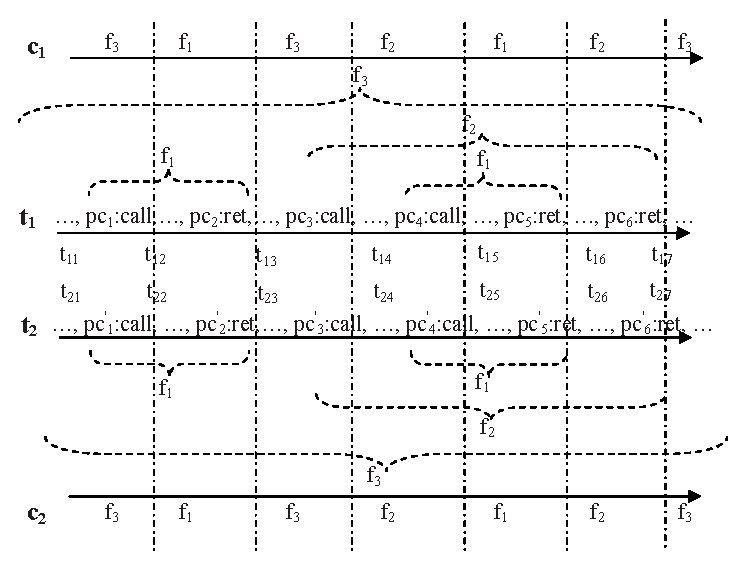
\includegraphics[width=0.5\textwidth]{fig/call1.eps}
\caption{Traces snippets generation and Traces partition }
\label{fig:calltrace}       % Give a unique label
\end{figure}

The call trace, which is the frame of instruction trace with other
instructions casted out, provides a higher and global view about the
expatiatory instruction trace. This could be very helpful for the
users who are dragged into the sea of instructions and cannot find
their way out.

Algorithm ~\ref{alg:similarity} shows how the similarity $s$ of two
traces $t_1$ and $t_2$ is calculated. At first, two call traces
$c_1$ and $c_2$ are generated from $t_1$ and $t_2$ respectively.
Then we compute the edit distance between $c_1$ and $c_2$. The
reconstructed edit distance $e$ for $t_2$ contains all the operation
of deletion, insertion and substitute that are performed on symbols
in $c_2$ to transform $c_2$ into $c_1$. We remove all the "call"s
and "return"s that are involved in $e$ from $c_1$. The new call
traces $c'_1$ generated from $c_1$ now only includes "call"s and
"return"s that appear in both $t_1$ and $t_2$ with positional
similarity and ordinal similarity. After that, we split $t_1$ and
$t_2$ into a number of subsequences according to the "call"s and
"return"s included in $c'_1$. We compare each pair of the
subsequences and calculate the final similarity of the two traces
using equation ~\ref{eq:sim}.

\begin{algorithm}[H]

\KwIn{traces $t_1$ and $t_2$}

\KwOut{Trace similarity $s$ and call trace edit distance $e$}

Generate call traces $c_1$ and $c_2$ from $t_1$ and $t_2$
respectively\;

$s_c=Lev_{c_1,c_2}(|c_1|,|c_2|)$\;

Reconstruct the edit sequence $e$ for $c_1$ and $c_2$\;

Build the best-matched common sequence $c$ based on $c_1$, $c_2$ and
$e$;

Split $t_1$ into a collection of subsequences $S_1$ based on $c$,
where $S_1=\{t_{1i}|1\leq i \leq |c'_1|\}$\;

Split $t_2$ into a collection of subsequences $S_2$ based on $c$,
where $S_2=\{t_{2i}|1\leq i \leq |c'_1|\}$ \;

$comm(t_1, t_2)=\empty$\;

\For{$i=1$ to $|c|$}{
    $comm(t_1, t_2) = comm(t_1, t_2) \cup comm(t_{1i}, t_{2i})$\;
}

$s={|comm(t_1, t_2|)}/{\max{(|t_1|,|t_{2}|)}}$\;

\caption{Similarity calculation for traces} \label{alg:similarity}
\end{algorithm}

The restricted edit sequence for $c_1$ is also provided to the user
for understanding the differences of the two traces. In our
implementation, the function names are also extracted from the
output of objdump, so that user knows where one calling path
diverges from another.

\section{Similarity Calculation Based-on instruction traces}
\subsection{Reducing the size of program traces}
Program trace is generated as a processor executes instructions and
jump around in code space. These instructions are Researchers
propose a number of algorithms used in version managing systems.
These algorithms are customized for source file comparing. Program
traces are instruction sequences and they have

\subsubsection{Grouping instructions Using Basic Blocks}
A basic block is a sequence of instructions with only one entry
point and one exit point. Whenever the first instruction is
executed, the rest of instructions in a same block are certainly
executed once in given order. Based on this observation, program
traces are partitioned into basic blocks, and instructions in a same
basic block are grouped together. Each basic block is considered as
a MACRO instruction. According to existing statistics results on
standard benchmarks, each basic block contains 5 instructions on
average. The number of MACRO instructions is about 1/5 of the number
of instructions in original trace. This optimization reduces the
sizes of traces.

\subsubsection{Intersecting traces}
Two executions may execute different instructions in different code
regions. This provides the opportunity to reduce the size of traces
by removing basic blocks that are only appears in one trace. Let
$B_t$ is the set of all basic blocks that visited by execution $t$,
Then set $B_{t1,t2} = B_{t1} \cap B_{t2}$ contains all the basic
blocks visited by both $t1$ and $t2$. $B_{t1} - B_{t1,t2}$ and
$B_{t2} - B_{t1,t2}$ contains all the unique basic blocks visited by
$t1$ and $t2$ respectively. Removing all the unique basic blocks
from the two traces also helps to reduce the length of the two
traces.


\section{Evaluation}
\subsection{Evaluation Method}
\label{sec:eval}

To verify our algorithm, we get two different execution traces of
same program using the popular dynamic instrument tool -
Pin~\cite{pin10} and full system simulator GEM4. In our experiments,
we compared the traces extracted from GEM5 to the ones obtained by
the Pin-tool. The configuration of the host machine for Pin-tool and
GEM5 simulator is given in the second row of table
~\ref{tab:sysconfig}. Even though the simulated x86-Linux is
different from the host machine in many aspects, we expect highly
similar traces for a same executable binary. This is because the
difference in micro-architecture dose not changes the order of
instructions in the same thread; however, in effect, they are not
exactly the same due to thread scheduling and synchronization. The
operating system images and compilers are all provided by the GEM5
team and we didn't make any modifications to these system softwares.
All the benchmarks are compiled with the "-static" options to make
sure that no differences will be introduced into the traces by using
different versions of dynamic loaded libraries.

\begin{table*}
\caption{System configuration} \label{tab:sysconfig} \centering
\begin{tabular}{|c|c|c|c|c|}
\hline Platform & CPU & Memory & OS & compiler \\
\hline Pin/GEM5 host system & Intel Xeon E5606/2.13GHz/4-core& 24 GB & Linux ubuntu 2.6.38 & gcc 4.5.2 \\
\hline GEM5-x86-linux & X86/2.0 GHz/4-core & 128 MB &  Linux 2.6.22.9.smp & gcc 4.5.2 \\
%\hline GEM5-Arm-linux & Arm... , 2 GHz, 1MB L2 & 128 MB &  Linux.. & gcc.xx \\
%\hline GEM5-Alpha-linux & Alpha/2.0 GHz/4-core & 128 MB &  Linux 2.6.13.smp & gcc 3.4.3 \\
\hline
\end{tabular}
\end{table*}

We use the standard multi-thread benchmarks to evaluate our
approach, and all of the used programs are selected from
SPLASH2~\cite{splash295}. All the benchmarks are compiled using a
same compiler and each binary is executed in both the host machine
and the simulated full system in GEM5 with an operating system
image. The features of the benchmarks we used are listed in table
~\ref{tab:benchmark}.

\begin{table*}
\caption{Benchmarks} \label{tab:benchmark} \centering
\begin{tabular}{|c|c|c|}
\hline Benchmark & Description & Group\\
\hline fft & A 1-D version of six-step FFT algorithm. & 1 \\
\hline lu-non & Dense matrix factoring kernel. & 1\\
\hline radix & Integer radix sort kernel. & 2 \\
\hline lu-con & Dense matrix factoring kernel. &  2\\
\hline FMM & Body interaction simulation. & 3\\
\hline Ocean & Large-scale ocean movements simulation. & 3\\
\hline Ocean-non & Large-scale ocean movements simulation. & 3\\
\hline
\end{tabular}
\end{table*}

Figure ~\ref{fig:x86_sis_sim} shows the calculated similarity(given
by equation ~\ref{eq:sim}) between two traces collected by hacked
GEM5 and Pin-tool respectively. All the GEM5 traces are collected
when the benchmarks are started and run separately and individually
in the simulated full system at different time. It shows that the
traces collected using GEM5 are much similar to the ones collected
by the Pin-tool. Though the the similarity of call traces is as high
as up to 98\% for most benchmarks, the instruction traces exhibit a
relative low similarity around 85\%. The reason for this is that the
hacked GEM5 only starts to generate traces after instruction
patterns are captured. Hence, the instructions executed at the
startup phase before the main function are not included in the GEM5
traces, which add up to about 10 thousands in total. Meanwhile, we
found that the difference between C-X-S and C-X-P is slightly
enlarged as the number of threads increases. In order to find out
the differences for the two call traces, the edit sequence for C-X-S
and C-X-P is rebuilt using our analysis tool. From the edit
sequence, we found the benchmarks with multiple threads spent much
longer time at the synchronization points than their sequential
versions. The threads, which run faster than others are scheduled
out and in from time to time, execute a number of instructions to
check the status of barriers. That is why we observed high
similarities for call traces on one side and low similarities for
instruction traces on the other side.

\begin{figure*}
\centering
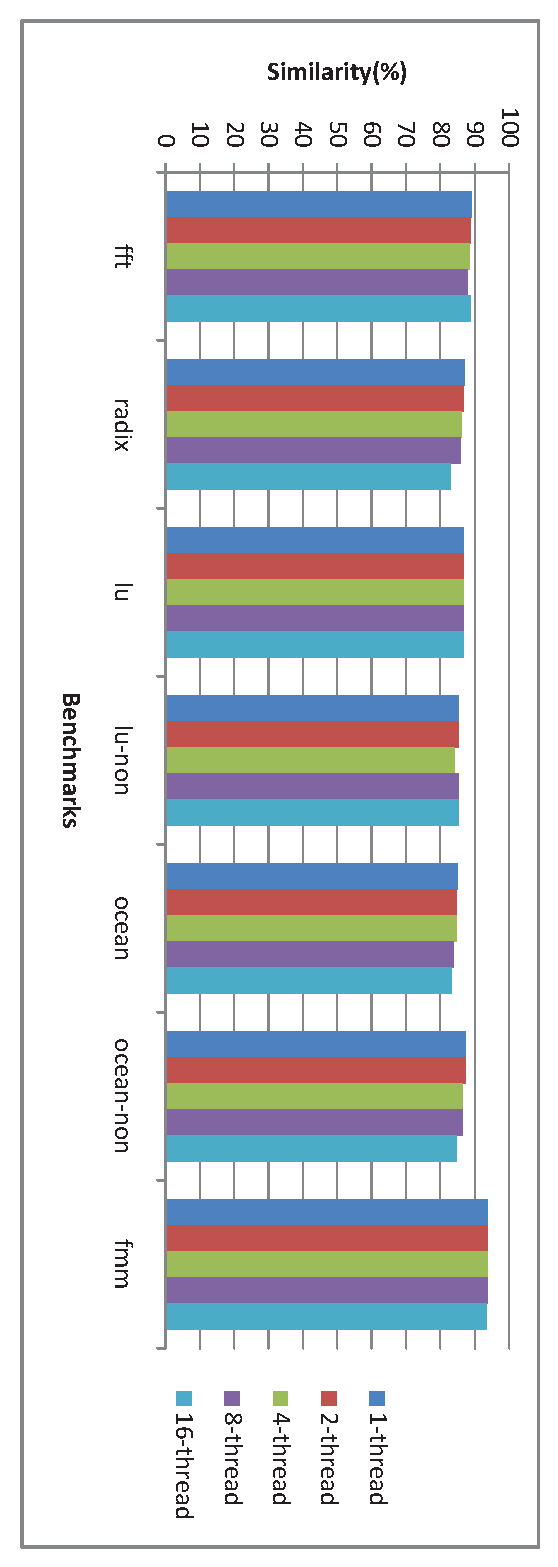
\includegraphics[width=0.21\textwidth, angle=90]{fig/x86_s_sim1.eps}
\caption{Instruction trace similarity for I-X-S and I-X-P}
\label{fig:x86_sis_sim}       % Give a unique label
\end{figure*}




\section{Conclusion}
races record all the information about a program's execution in the
form of instruction sequences. They are for dynamic behavior
understanding and trace driven simulation. In this paper, we propose
a generic approach to extract traces for applications in full system
simulation environments. Traces are extracted for each application
from the instruction stream blended with instructions from OS
modules and other applications. Each thread in a given application
is identified by an instruction pattern without inspecting the
internal state of the OS. Our approach can be applied to existing
full system simulators with no changes to the compiler. We also
present an effective and efficient algorithm to measure the
differences of two traces. This algorithm computes edit distances
for traces and reconstruct edit sequences, so that we know how
similar the two traces are and where the difference is. It will be
very helpful for the users who need to analyze and understanding
very large traces composed of millions of instructions. We
implemented our instruction extraction approach in the simulator
GEM5 and performed a number of experiments on the simulated full
system X86-Linux and Alpha-Linux. Experimental results show that our
approaches are effective and efficient to extract and compare traces
in full system simulation environments.


% if have a single appendix:
%\appendix[Proof of the Zonklar Equations]
% or
%\appendix  % for no appendix heading
% do not use \section anymore after \appendix, only \section*
% is possibly needed

% use appendices with more than one appendix
% then use \section to start each appendix
% you must declare a \section before using any
% \subsection or using \label (\appendices by itself
% starts a section numbered zero.)
%


\appendices
\section{Proof of the First Zonklar Equation}
Appendix one text goes here.

% you can choose not to have a title for an appendix
% if you want by leaving the argument blank
\section{}
Appendix two text goes here.Appendix two text goes here.Appendix two text goes here.Appendix two text goes here.Appendix two text goes here.Appendix two text goes here.Appendix two text goes here.Appendix two text goes here.Appendix two text goes here.Appendix two text goes here.Appendix two text goes here.Appendix two text goes here.Appendix two text goes here.Appendix two text goes here.Appendix two text goes here.Appendix two text goes here.Appendix two text goes here.Appendix two text goes here.Appendix two text goes here.Appendix two text goes here.Appendix two text goes here.Appendix two text goes here.Appendix two text goes here.Appendix two text goes here.Appendix two text goes here.


% use section* for acknowledgement
\ifCLASSOPTIONcompsoc
  % The Computer Society usually uses the plural form
  \section*{Acknowledgments}
\else
  % regular IEEE prefers the singular form
  \section*{Acknowledgment}
\fi


The authors would like to thank...The authors would like to thank...The authors would like to thank...The authors would like to thank...The authors would like to thank...The authors would like to thank...The authors would like to thank...The authors would like to thank...The authors would like to thank...The authors would like to thank...The authors would like to thank...The authors would like to thank...The authors would like to thank...


% Can use something like this to put references on a page
% by themselves when using endfloat and the captionsoff option.
\ifCLASSOPTIONcaptionsoff
  \newpage
\fi



% trigger a \newpage just before the given reference
% number - used to balance the columns on the last page
% adjust value as needed - may need to be readjusted if
% the document is modified later
%\IEEEtriggeratref{8}
% The "triggered" command can be changed if desired:
%\IEEEtriggercmd{\enlargethispage{-5in}}

% references section

% can use a bibliography generated by BibTeX as a .bbl file
% BibTeX documentation can be easily obtained at:
% http://www.ctan.org/tex-archive/biblio/bibtex/contrib/doc/
% The IEEEtran BibTeX style support page is at:
% http://www.michaelshell.org/tex/ieeetran/bibtex/
%\bibliographystyle{IEEEtran}
% argument is your BibTeX string definitions and bibliography database(s)
%\bibliography{IEEEabrv,../bib/paper}
%
% <OR> manually copy in the resultant .bbl file
% set second argument of \begin to the number of references
% (used to reserve space for the reference number labels box)

\bibliographystyle{IEEEtran}
\bibliography{references}


%\begin{thebibliography}{1}
%\bibitem{}




%\bibitem{IEEEhowto:kopka}
%This is an example of a book reference
%H. Kopka and P.W. Daly, \emph{A Guide to {\LaTeX}}, third ed. Harlow, U.K.: Addison-Wesley, 1999.


%This is an example of a Transactions article reference
%D.S. Coming and O.G. Staadt, "Velocity-Aligned Discrete Oriented Polytopes for Dynamic Collision Detection," IEEE Trans. Visualization and Computer Graphics, vol.14, no.1, pp. 1-12, Jan/Feb 2008, doi:10.1109/TVCG.2007.70405.

%This is an example of a article from a conference proceeding
%H. Goto, Y. Hasegawa, and M. Tanaka, "Efficient Scheduling Focusing on the Duality of MPL Representation," Proc. IEEE Symp. Computational Intelligence in Scheduling (SCIS '07), pp. 57-64, Apr. 2007, doi:10.1109/SCIS.2007.367670.

%This is an example of a PrePrint reference
%J.M.P. Martinez, R.B. Llavori, M.J.A. Cabo, and T.B. Pedersen, "Integrating Data Warehouses with Web Data: A Survey," IEEE Trans. Knowledge and Data Eng., preprint, 21 Dec. 2007, doi:10.1109/TKDE.2007.190746.

%Again, see the IEEEtrans_HOWTO.pdf for several more bibliographical examples. Also, more style examples
%can be seen at http://www.computer.org/author/style/transref.htm
%\end{thebibliography}

% biography section
%
% If you have an EPS/PDF photo (graphicx package needed) extra braces are
% needed around the contents of the optional argument to biography to prevent
% the LaTeX parser from getting confused when it sees the complicated
% \includegraphics command within an optional argument. (You could create
% your own custom macro containing the \includegraphics command to make things
% simpler here.)
%\begin{biography}[{\includegraphics[width=1in,height=1.25in,clip,keepaspectratio]{mshell}}]{Michael Shell}
% or if you just want to reserve a space for a photo:

\begin{IEEEbiography}{Michael Shell}
Biography text here.
\end{IEEEbiography}

% if you will not have a photo at all:
\begin{IEEEbiographynophoto}{John Doe}
Biography text here.Biography text here.Biography text here.Biography text here.Biography text here.Biography text here.Biography text here.Biography text here.Biography text here.Biography text here.Biography text here.Biography text here.Biography text here.Biography text here.Biography text here.Biography text here.Biography text here.Biography text here.Biography text here.Biography text here.Biography text here.Biography text here.Biography text here.Biography text here.Biography text here.Biography text here.Biography text here.Biography text here.Biography text here.Biography text here.Biography text here.Biography text here.
\end{IEEEbiographynophoto}

% insert where needed to balance the two columns on the last page with
% biographies
%\newpage

\begin{IEEEbiographynophoto}{Jane Doe}
Biography text here.Biography text here.Biography text here.Biography text here.Biography text here.Biography text here.Biography text here.Biography text here.Biography text here.Biography text here.Biography text here.Biography text here.Biography text here.Biography text here.Biography text here.Biography text here.Biography text here.Biography text here.Biography text here.Biography text here.Biography text here.Biography text here.Biography text here.Biography text here.Biography text here.Biography text here.Biography text here.Biography text here.
\end{IEEEbiographynophoto}

% You can push biographies down or up by placing
% a \vfill before or after them. The appropriate
% use of \vfill depends on what kind of text is
% on the last page and whether or not the columns
% are being equalized.

%\vfill

% Can be used to pull up biographies so that the bottom of the last one
% is flush with the other column.
%\enlargethispage{-5in}



% that's all folks
\end{document}
